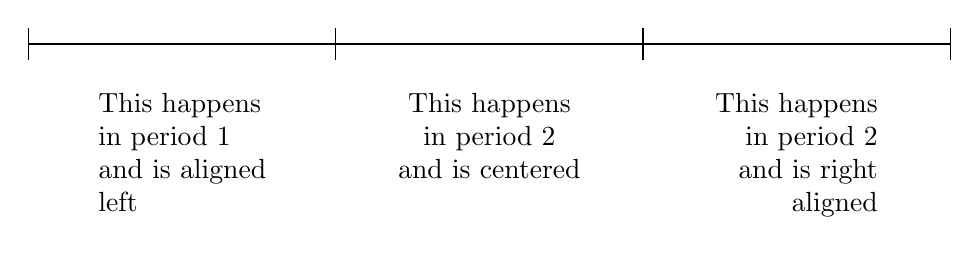
\begin{tikzpicture}[xscale=1.3]
  \draw [thick] (0,0) -- (9,0);
  \draw (0,-.2) -- (0, .2);
  \draw (3,-.2) -- (3, .2);
  \draw (6,-.2) -- (6, .2);
  \draw (9,-.2) -- (9, .2);
  \node[align=left, below] at (1.5,-.5)%
       {This happens\\in period 1\\and is aligned\\ left};
  \node[align=center, below] at (4.5,-.5)%
       {This happens\\in period 2\\and is centered};
  \node[align=right, below] at (7.5,-.5)%
       {This happens\\in period 2\\and is right\\aligned};
\end{tikzpicture}
